
\documentclass{beamer}
\usepackage[orientation=portrait, size=a1, scale=1.4, debug]{beamerposter}
\usetheme{unn}

\usepackage{cmbright}

\usepackage{fontspec}

\setmainfont{Times New Roman}
\setromanfont{Times New Roman}
\setsansfont{Times New Roman}

\usepackage{polyglossia}
\setmainlanguage{russian}
\usepackage{csquotes}

\usepackage{booktabs}
\usepackage{ragged2e}

\usepackage[backend=biber,
            movenames=false,
            maxnames=4,
            style=gost-numeric,
            sorting=nty,
            autolang=other]{biblatex}
						
%\newfontfamily\cyrillicfonttt{lmmonolt10-regular.otf}
%\newfontfamily\cyrillicfontsf{lmsans10-regular.otf}						
					
\addbibresource{bibliography.bib}

\DeclareMathOperator{\re}{\operatorname{Re}}

\title{Эффективные методы глобальной оптимизации
для решения задач оптимального управления
}
\author{К.А. Баркалов \and М.А. Кочеганова \and С.А. Бевзюк \and А.А. Федюков}
\institute{ННГУ им. Н.И. Лобачевского}
\setlength{\abovedisplayskip}{3pt}
\setlength{\belowdisplayskip}{3pt}

\begin{document}
\begin{frame}[t]
    \begin{columns}[t]
        \begin{column}[t]{0.48\paperwidth}
            \begin{block}{Задача поиска $H_{\infty}$-динамического регулятора}
              Рассматривается задача поиска $H_{\infty}$ -динамического регулятора для обратного маятника с подвижным основанием.
							\begin{equation}\label{eq:system}
                \dot{x}=A x + B_1 v + B_2 u
              \end{equation}
							Известно \cite{synthesisControlBook}, что для существования регулятора с наименьшим уровнем гашения возмущений $\gamma>0$ необходимо и достаточно, чтобы существовала матрица $X=X^T>0$, удовлетворяющая  двум матричным неравенствам, одно из которых не является выпуклым, т.к. зависит от обратной матрицы $X^{-1}$:
							\begin{equation}\label{eq:matrix_1}
                W_{P}^T 
								\begin{bmatrix}
                  \quad A_{0}^T X + X A_0 & X B_0 & C_{0}^T \\
                  B_{0}^T X & -\gamma I & 0 \\
									C_0  & 0 & -\gamma I \quad \\
                \end{bmatrix}
								W_P
                < 0
              \end{equation}
							\begin{equation}\label{eq:matrix_2}
                W_{R}^T 
								\begin{bmatrix}
                  \quad X^{-1} A_{0}^T + A_0 X^{-1} & B_0 & X^{-1} C_{0}^T \quad  \\
                  B_{0}^T & -\gamma I & 0 \\
									C_0 X^{-1} & 0 & -\gamma I\\
                \end{bmatrix}
								W_R
                < 0
              \end{equation}
							Возникает задача поиска минимального значения $\gamma$  при ограничениях \eqref{eq:matrix_1} и \eqref{eq:matrix_2}.
Причем неравенство \eqref{eq:matrix_2} не может быть представлено в виде линейного матричного неравенства, т.е. данную задачу нельзя решить стандартными методами выпуклой оптимизации в сочетании
с методами решения линейных матричных неравенств, реализованными,
например, в MATLAB Robust Toolbox. Требуется использование
методов, обладающих сходимостью к глобальному экстремуму.
						
          \end{block}
            \begin{block}{Задача глобальной оптимизации}
              Общая постановка задачи глобальной оптимизации с ограничениями:
              \begin{displaymath}
                \varphi(y^*)=\min\{\varphi(y):y\in D\}, D=\{x\in \mathbf{R}^n: g_j(x) \leqslant 0, j=\overline{1,m}\}
              \end{displaymath}
              Предполагается, что все функции задачи удовлетворяют условию Липшица:
              \begin{displaymath}
              |f(y_1)-f(y_2)|\leqslant L\Vert y_1-y_2\Vert,y_1,y_2\in D,0<L<\infty
              \end{displaymath}

              Целевая функция и ограничения могут быть невыпуклы, многоэкстремальны, недифференцируемы.
            \end{block}
            \begin{block}{Метод глобальной оптимизации}
              Задача оптимизации решается Алгоритмом Глобального Поиска (АГП), предложенным Р.Г. Стронгиным \cite{strOptBook}. При этом решение многомерной задачи сводится к решению эквивалентной ей одномерной задачи с помощью развертки Пеано, отображающей отрезок $[0,1]$  на гиперкуб $D$.

              Общая схема одной итерации одномерного метода:
              \begin{enumerate}
                \justifying
                \item Упорядочить точки предшествующих испытаний в порядке возрастания их координат: \(a=x_{0}<...<x_{i}<...<x_{k}=b\).
                \item Вычислить для каждого интервала \((x_{i-1};x_{i}),1\leq i\leq k\)  характеристику \(R(i)\) .
                \item Определить интервал \((x_{t-1};x_{t})\) , которому соответствует максимальная характеристика \(R(t)=\max\{R(i),1\leq i\leq k\}\).
                \item Провести следующее испытание в точке \(x^{k+1}=d(t)\in (x_{t-1};x_{t})\) , где \(d(t)\)  — правило размещения точки следующего испытания в интервале с номером \(t\).
                \item Проверить выполнение критерия остановки \(x_{t}-x_{t-1}<\varepsilon\).
              \end{enumerate}
              Подробное описание АГП, а также специальной схемы учёта ограничений (без использования штрафных функций) можно найти в \cite{strOptBook}.

              \begin{minipage}[t]{.48\textwidth}
              \begin{figure}
                  \centering
                  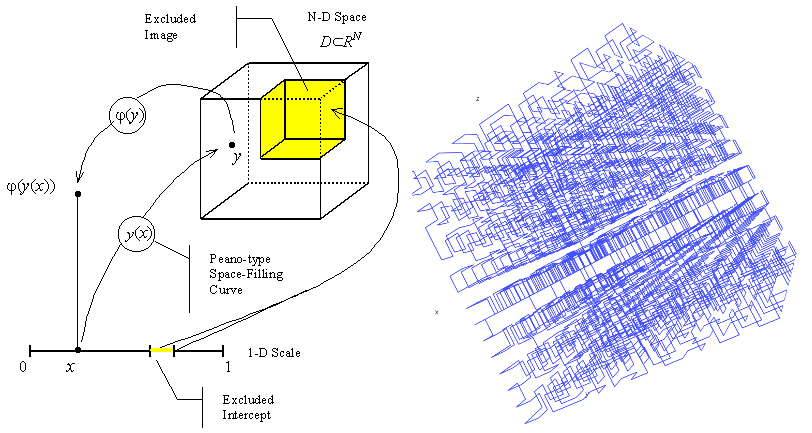
\includegraphics[scale=1.27]{images/peano.png}
              \end{figure}
              \end{minipage}
            \end{block}
        \end{column}
        \begin{column}[t]{0.48\paperwidth}
          \begin{block}{Параллельные версии метода оптимизации}
            Существует несколько способов распареллеливания алгоритма глобального поиска (АГП):
            \begin{itemize}
              \justifying
              \item Распараллеливание по характеристикам в рамках системы с общей памятью.
              На шаге 2 вместо одного интервала выбираются \(p\) интервалов с наилучшими характеристиками и в них параллельно проводятся испытания.
              \item Распараллеливание по развёрткам в рамках системы с раздельной памятью. На каждом узле системы работает копия метода, использующая
              уникальную развёртку. Копии метода обмениваются многомерными точками, однако одномерные прообразы этих точек различны для каждого метода.
              При использовании \(L\) развёрток каждый метод дополнительно получает \(L-1\) точку в свою поисковую информацию на каждой итерации, что
              ускоряет его сходимость.
              \item Сочетание указанных выше подходов.
            \end{itemize}
          В \cite{optParallelBook} перечисленные схемы описаны более подробно.
          \end{block}
          \begin{block}{Результаты}
						
						Решена модельная задача, связанная со стабилизацией плоского перевернутого маятника с подвижным основанием.
Найдены параметры регулятора $\theta$ и соответствующее им минимальное значение уровня гашения возмущений $\gamma$. 
Размерность (число параметров) возникающей при этом задачи глобальной оптимизации $N=7$.

          \begin{table}[h]
            \caption{Сравнение последовательного и параллельного алгоритма}
            \label{tab:Results}
            \begin{tabular}{l|c}
						  \hline
              Алгоритм & Время решения задачи (сек.) \\ 
              \hline
              Последовательный алгоритм  &  125 \\
              Параллельный алгоритм (4 ядра)  &  82 \\
              \hline
							Ускорение & 1.5 \\
							\hline
            \end{tabular}
           \end{table}
					
					Эксперименты проводились в системе Globalizer \cite{globalizer} на узле кластера <<Лобачевский>>, CPU Intel Core i7 (3.6 GHz).
          \end{block}
          \begin{block}{Дальнейшая работа}
						\begin{enumerate}
                \item В процессе решения задачи обнаружен эффект резкого роста константы Липшица для функций ограничений задачи, что существенно затрудняет поиск глобального экстремума.
Планируется разработать подход к учету и обработке подобных ситуаций (идентификация и исключение из рассмотрения подобластей, в которых происходит скачкообразное изменение значений функции).

                \item Вычисление ограничений задачи сводится к обращению матрицы $X$ и поиску собственных чисел матриц из правой части ограничений \eqref{eq:matrix_1}, \eqref{eq:matrix_2}. Планируется распараллелить данные операции, что будет актуальным при поиске динамических регуляторов для задач вида \eqref{eq:system} большой размерности.
						\end{enumerate}
          \end{block}
          \begin{block}{Литература}
            \printbibliography
          \end{block}
        \end{column}
    \end{columns}
\end{frame}
\end{document}
